\section{Tools used}
\label{sec:tools}

\verb|Python| was our language of choice to implement our tool to predict if a 
tweet will be retweeted or not. Multiple libraries were used:
\begin{itemize}
	\item matplotlib: to plot 2D graphs of the ROC curve.
	\item nltk: for stemming and various language processing functions and some 
		  classifiers.
	\item numpy: to use special array objects.
	\item scipy: for some numerical routines.
	\item scikit-learn: for some classifiers.
	\item twython: to extract tweets from Twitter using their API.
\end{itemize}

Due to some libraries being not compatible with \verb|Python 3|, we had to 
stick with \verb|Python 2|.

We were able to develop a comprehensive tool that is easy to extend by taking 
advantage of object oriented programming. Adding new features or new 
classifiers can be done very easily thanks to the concept of inheritance.

The figure \ref{fig:architecture} shows the global architecture of the 
interesting part of the code.

\begin{figure}[!h]
\centering
 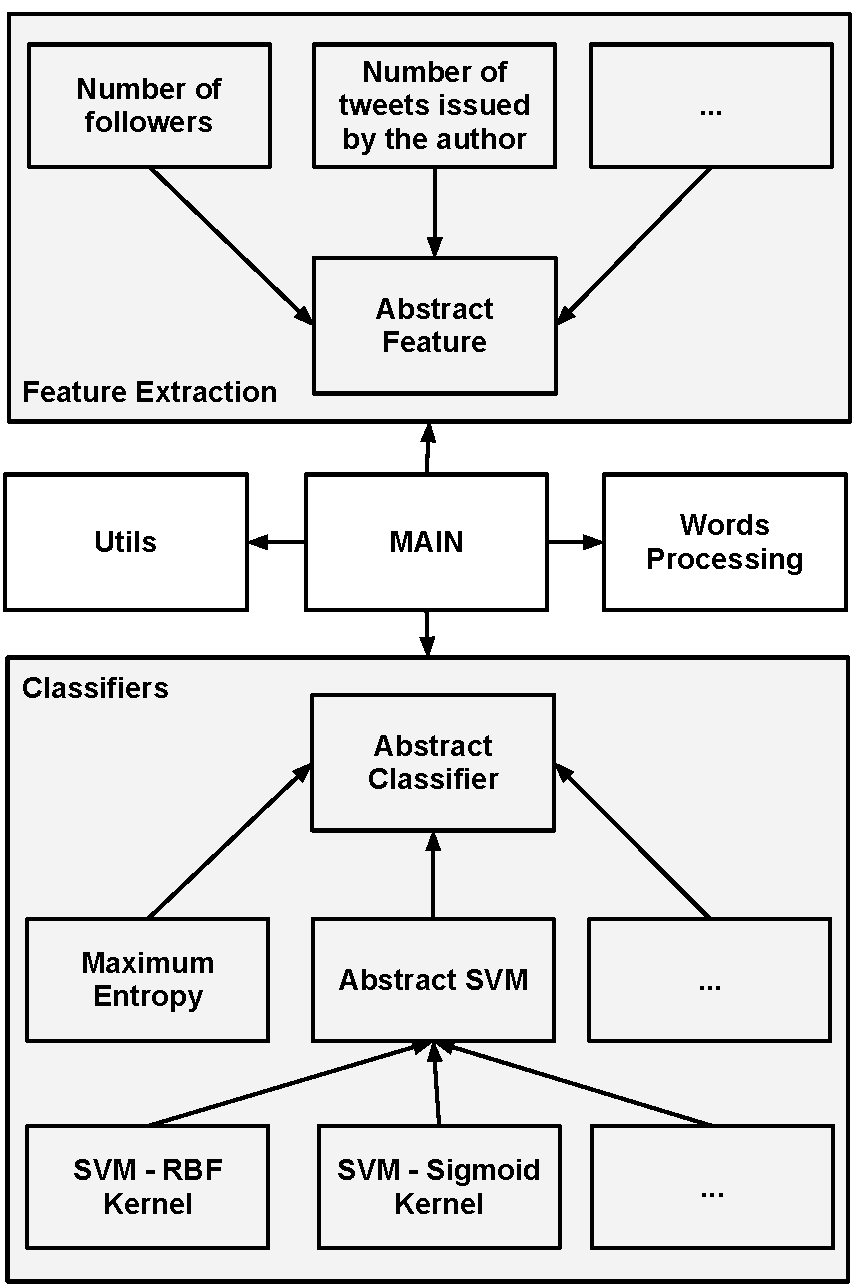
\includegraphics[width=0.9\columnwidth]{img/architecture.pdf}
\caption{Source code architecture}
\label{fig:architecture}
\end{figure}

Our tool is able to perform various tasks such as classification using numerous 
classifiers and features, algorithm tournament and cross-validation. It is also 
able to plot ROC curve and Decision Trees, randomizing the dataset and taking 
the advantage of multiprocessing for performing hard computing tasks.

In order to let the scientific community, or any people, use it, we released it 
under the terms of the permissive BSD license. Being written in \verb|Python|, 
it is available for any operating system on which \verb|Python| can run. We, 
however, only tested it on Linux.
